% !TeX spellcheck = ru_RU
% !TeX spellcheck = en_US
\documentclass{vkr-slides-style}
\usepackage{listings}

\filltitle{
    % Ваше ФИО.
    author = {Михайлов Илья Игоревич},
    % Нельзя оставлять пустые строки.
    % Ваше сокращённое именование, будет показываться слева внизу слайда.
    authorShort = {Михайлов Илья},
    %
    % Официальное название ВКР.
    title = {Динамическая бинарная трансляция в RISC-V с помощью Instrew},
    %
    % Короткое название ВКР, будет снизу по центру слайда.
    titleShort = {RISC-V Instrew},
    %
    % Научный руководитель.
    advisor = {ассистент кафедры системного программирования, Косарев~Д.~С.},
    %
    % Консультант (если есть). Если нет, оставьте пустые фигурные скобки.
    consultant = {
    },
    %
    % Дата доклада.
    date = {28.11.2023}
}

\begin{document}

\makeslidestitle

\begin{frame}
    \frametitle{Введение}
    \begin{itemize}
        %     \item Тут кратко и по делу рассказываете, что именно хотите сделать
        %     \item Обозначьте отчуждаемый результат (что это будет --- приложение, инструмент, библиотека, ...), открыт ли код
        %     \item Должно быть понятно, в чём решаемая проблема, почему нельзя взять готовое решение, и кому это нужно (желательно с точностью до конкретной компании, а не вообще --- если работодатель предложил или утвердил тему, укажите это тут)
        %     \item Должен быть понятен объём работы (почему это диплом)
        %     \item Должно быть понятно, при чём тут СП\footnote{Ещё не поздно защищаться на ИАС или информатике.}
        \item Бинарные трансляторы являются популярными инструментами для анализа кода, профиляции и эмуляции, важным классом которых являются динамические бинарные трансляторы (далее --- ДБТ)
              % Бинарная трансляция -- это актуально, но бинарная трансляция с лифтингом двоичного кода в LLVM IR -- это еще и круто.
        \item В качестве промежуточного представления для ДБТ хорошо использовать LLVM IR
              \begin{itemize}
                  \item Тулчейн LLVM позволяет проводить качественные оптимизации
              \end{itemize}
              %Хотим добавить поддержку архитектуры RISC-V для такого ДБТ c поднятием в LLVM IR
        \item Instrew является ДБТ с поднятием кода в LLVM IR, но нет поддержки RISC-V, как хост-архитектуры
        \item Результатом работы является добавление поддержки архитектуры RISC-V для ДБТ Instrew с открытым исходным кодом
        \item В связи с наличием процессорно-специфических и низкоуровневых деталей реализации, задача является довольно трудоемкой
              % \item (Что по сути является классической задачей программной инженерии)
    \end{itemize}
\end{frame}

\begin{frame}
    \frametitle{Постановка задачи}
    \textbf{Цель:} Добавить поддержку архитектуры RISC-V для ДБТ Instrew.

    \vspace{5mm}
    \textbf{Задачи:}
    \begin{enumerate}
        \item Выполнить обзор динамических бинарных трансляторов и сравнить их с Instrew
              % \item Спроектировать то-то
        \item Выполнить обзор архитектуры Instrew
        \item Реализовать минимальную функциональность для запуска Instrew
              на RISC-V:
              \begin{itemize}
                  \item Добавить процессорно-специфические патчи в minilibc и другие компоненты
                  \item Реализовать функции, связанные с RISC-V ABI
              \end{itemize}
        \item Провести тестирование
              % (например на SPEC CPU 2017)
    \end{enumerate}
\end{frame}

\begin{frame}
    \frametitle{Обзор}
    \begin{itemize}
        \item Динамические бинарные трансляторы:
              \begin{itemize}
                  \item QEMU
                  \item Box64
                  \item Rosetta 2
                  \item Valgrind
              \end{itemize}
        \item Динамические бинарные трансляторы с поднятием в LLVM IR:
              \begin{itemize}
                  \item Remill + McSema
                  \item Instrew + Rellume
                  \item DBILL
              \end{itemize}
    \end{itemize}
\end{frame}

\begin{frame}
    \frametitle{Архитектура Instrew}
    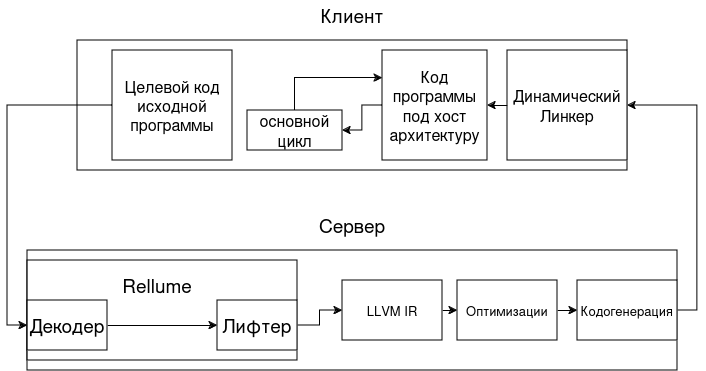
\includegraphics[width=370pt]{pictures/instrew.drawio.png}
\end{frame}

\begin{frame}[fragile]
    \frametitle{Пример (1/4)}
    \begin{lstlisting}[caption={objdump -d exit.S}, frame=single, breaklines, basicstyle=\footnotesize]
        Disassembly of section .text
        000000000001010c <_start>:
        1010c:       4501                    li      a0,0
        1010e:       05e00893                li      a7,94
        10112:       00000073                ecall
        10116:       a001                    j       10116 <_start+0xa>

    \end{lstlisting}

\end{frame}
\begin{frame}[fragile]
    \frametitle{Пример (2/4)}
    \vspace{-4pt}
    \begin{lstlisting}[caption={./build/server/instrew --dumpir=lift ./test/riscv64/exit}, frame=single, breaklines, basicstyle=\footnotesize]
    define void @S0_1010c(ptr addrspace(1) noalias nocapture align 16 dereferenceable(400) %0) #0 {
      %2 = getelementptr i8, ptr addrspace(1) %0, i64 0
        .............
      %66 = getelementptr i8, ptr addrspace(1) %0, i64 512
      %67 = load i64, ptr addrspace(1) %0, align 8
      br label %68
    68:                                               ; preds = %1
      store i64 65814, ptr addrspace(1) %0, align 8
      store i64 0, ptr addrspace(1) %13, align 8
      store i64 94, ptr addrspace(1) %20, align 8
      call void @syscall_rv64(ptr addrspace(1) %0)
      %69 = load i64, ptr addrspace(1) %0, align 8
      br label %70
    70:                                               ; preds = %68
      %71 = phi i64 [ %69, %68 ]
    \end{lstlisting}
\end{frame}

\begin{frame}[fragile]
    \frametitle{Пример (3/4)}
    \begin{lstlisting}[caption={./build/server/instrew --dumpir=codegen ./test/riscv64/exit}, frame=single, breaklines, basicstyle=\footnotesize]
        declare void @syscall_rv64(ptr addrspace(1))
        ; Function Attrs: null_pointer_is_valid
        define void @S0_1010c(ptr addrspace(1) noalias nocapture align 16 dereferenceable(400) %0) #0 {
          br label %2
        2:                                                ; preds = %1
          %3 = getelementptr inbounds i8, ptr addrspace(1) %0, i64 144
          %4 = getelementptr inbounds i8, ptr addrspace(1) %0, i64 88
          store i64 65814, ptr addrspace(1) %0, align 16
          store i64 0, ptr addrspace(1) %4, align 8
          store i64 94, ptr addrspace(1) %3, align 16
          call void @syscall_rv64(ptr addrspace(1) %0)
          br label %5
        5:                                                ; preds = %2
          ret void
    \end{lstlisting}
\end{frame}

\begin{frame}[fragile]
    \frametitle{Пример (3/4)}
    \begin{lstlisting}[caption={./build/server/instrew --dumpobj ./test/riscv64/exit}, frame=single, breaklines, basicstyle=\footnotesize]
        0000000000000000 <S0_1010c>:
   0:   ff010113                addi    sp,sp,-16
   4:   00113423                sd      ra,8(sp)
   8:   000105b7                lui     a1,0x10
   c:   1165859b                addiw   a1,a1,278 # 10116 <S0_1010c+0x10116>
  10:   00b53023                sd      a1,0(a0)
  14:   04053c23                sd      zero,88(a0)
  18:   05e00593                li      a1,94
  1c:   08b53823                sd      a1,144(a0)
  20:   00000097                auipc   ra,0x0
  24:   000080e7                jalr    ra # 20 <S0_1010c+0x20>
  28:   00813083                ld      ra,8(sp)
  2c:   01010113                addi    sp,sp,16
  30:   00008067                ret

    \end{lstlisting}
\end{frame}

\begin{frame}[fragile]
    \frametitle{Реализация (1/3)}
    \begin{lstlisting}[caption={Релокация}, frame=single, breaklines, basicstyle=\footnotesize]
        uint64_t syma = (uintptr_t) sym + patch_data->addend;
        uint64_t pc = patch_data->patch_addr;
        int64_t prel_syma = syma - (int64_t) pc;

        case R_RISCV_32_PCREL:

        if (!rtld_elf_signed_range(prel_syma, 32, "R_RISCV_32_PCREL"))
           return -EINVAL;
        rtld_blend(tgt, 0xffffffffff, prel_syma);
        break;
    \end{lstlisting}
\end{frame}


\begin{frame}[fragile]
    \frametitle{Реализация (2/3)}
    \vspace{-12pt}
    \begin{lstlisting}[caption={Заголовок}, frame=single, breaklines, basicstyle=\footnotesize]
        ASM_BLOCK(
            .text;
            .global _start;
            .type _start, %function;
        _start:
            .weak __global_pointer$;
            .hidden __global_pointer$;
            .option push;
            .option norelax;
            lla gp, __global_pointer$;
            .option pop;
            mv a0, sp;
            .weak _DYNAMIC;
            .hidden _DYNAMIC;
            lla a1, _DYNAMIC;
            andi sp, sp, -16;
            tail __start_main;  );
    \end{lstlisting}
\end{frame}


\begin{frame}[fragile]
    \frametitle{Реализация (3/3)}
    \begin{lstlisting}[caption={Системный вызов}, frame=single, breaklines, basicstyle=\footnotesize]
        static size_t syscall2(int n, size_t a, size_t b)
        {
            register size_t a7 __asm__("a7") = n;
            register size_t a0 __asm__("a0") = a;
            register size_t a1 __asm__("a1") = b;
            __asm_syscall("r"(a7), "0"(a0), "r"(a1))
        }
    \end{lstlisting}
\end{frame}

\begin{frame}
    \frametitle{Заключение}
    %Тут уместно рассказать подробности по каждому пункту, но кратко.
    В результате работы были выполнены следующие задачи:
    \vspace{8pt}
    \begin{enumerate}
        \item Выполнен обзор архитектуры Instrew и других ДБТ
        \item Реализованы некоторые процессорно-специфические патчи
        \item Реализована эмуляция системных вызовов
        \item Реализованы архитектурно-специфичные ELF релокации
    \end{enumerate}
    \vspace{8pt}
    Протестировать Instrew на простых примерах не удалось, из-за сложности локализации ошибки в реализации релокаций
\end{frame}

\end{document}
